Antes de hablar de las versiones de TCP, hay algunos puntos que son necesarios explicar:
\subsubsection*{Slow Start (SS)}
Es un algoritmo que equilibra la velocidad de una conexión de red. Inicia gradualmente la cantidad de datos transmitidos hasta que encuentra la capacidad máxima de carga de la red. Equilibra la cantidad de datos que puede transmitir un remitente con la cantidad de datos que el receptor puede aceptar. Comienza con una Congestion Window Size (CWDN) y el valor se incrementa en uno por cada \texttt{ACK}. Es decir se dobla por cada \texttt{RTT}.
       
\begin{figure}[H]
\centering
  \begin{tikzpicture}
    \node [copy shadow={draw=gray,fill=gray,opacity=0.5,shadow xshift=-0.5ex,
           shadow yshift=-0.5ex},fill=white!20,draw=black,thick,font=\bfseries]
            {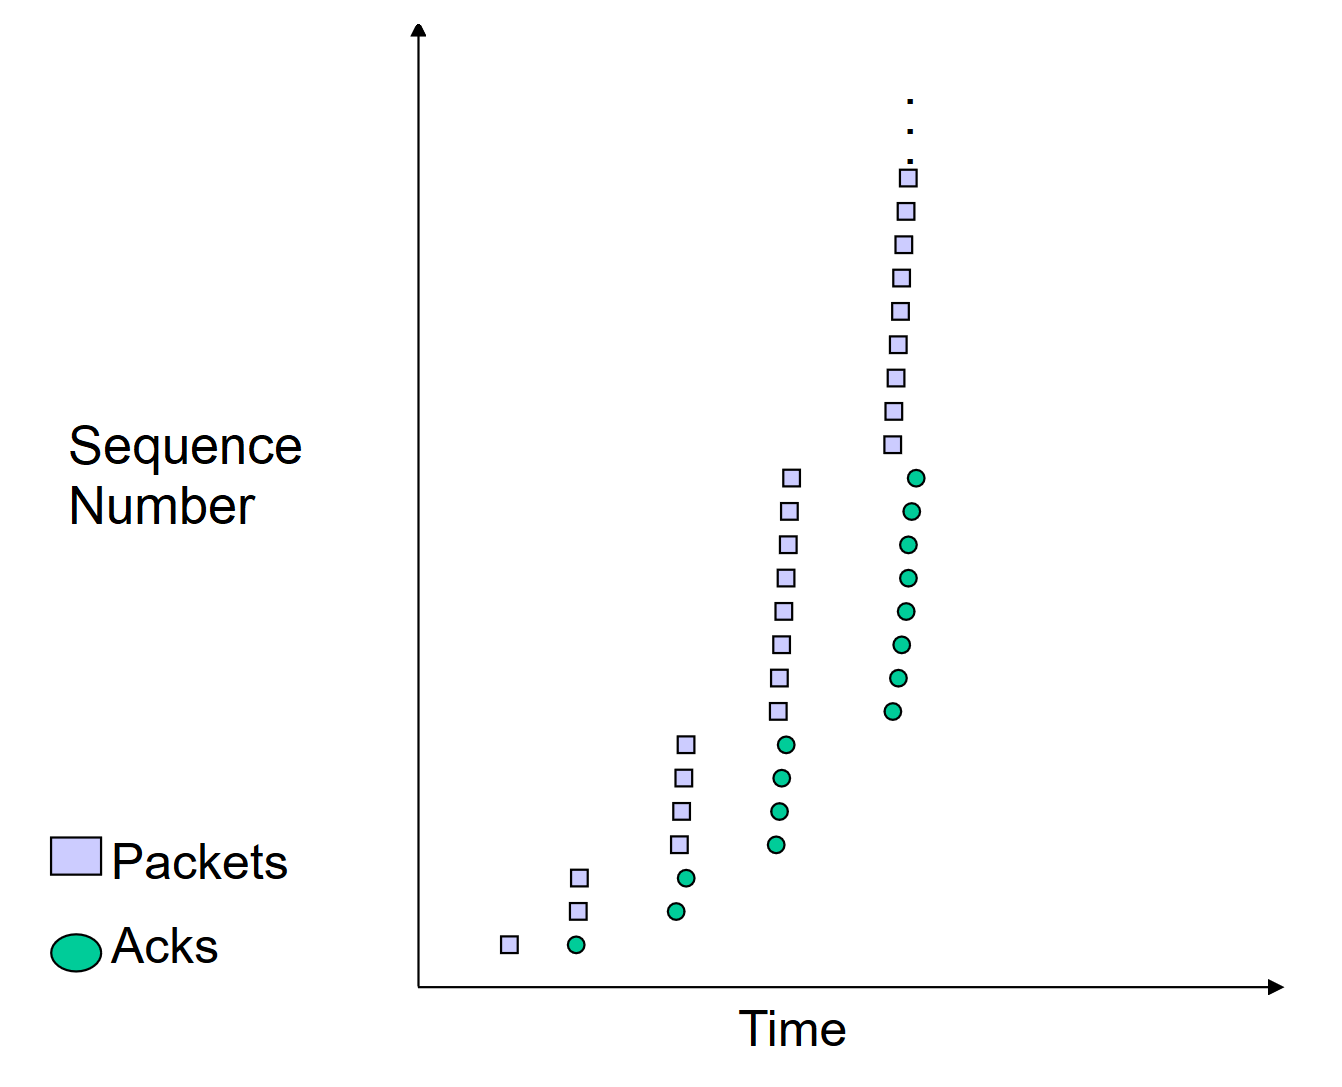
\includegraphics[page=1,scale=0.45]{SS.png}};
  \end{tikzpicture}
\caption{\textit{Presentación: Transport Layer: TCP Congestion Control $\&$ Buffer Management, Lilian Carroll, Slide 16}}
\end{figure}

\subsubsection*{Additive Increase, Multiplicative Decrease (AIMD)}
Es un algoritmo de control de feedback. Combina el incremento lineal de la ventana de congestión con una reduccion exponencial cuando se detecta congestión.

\begin{figure}[H]
\centering
  \begin{tikzpicture}
    \node [copy shadow={draw=gray,fill=gray,opacity=0.5,shadow xshift=-0.5ex,
           shadow yshift=-0.5ex},fill=white!20,draw=black,thick,font=\bfseries]
            {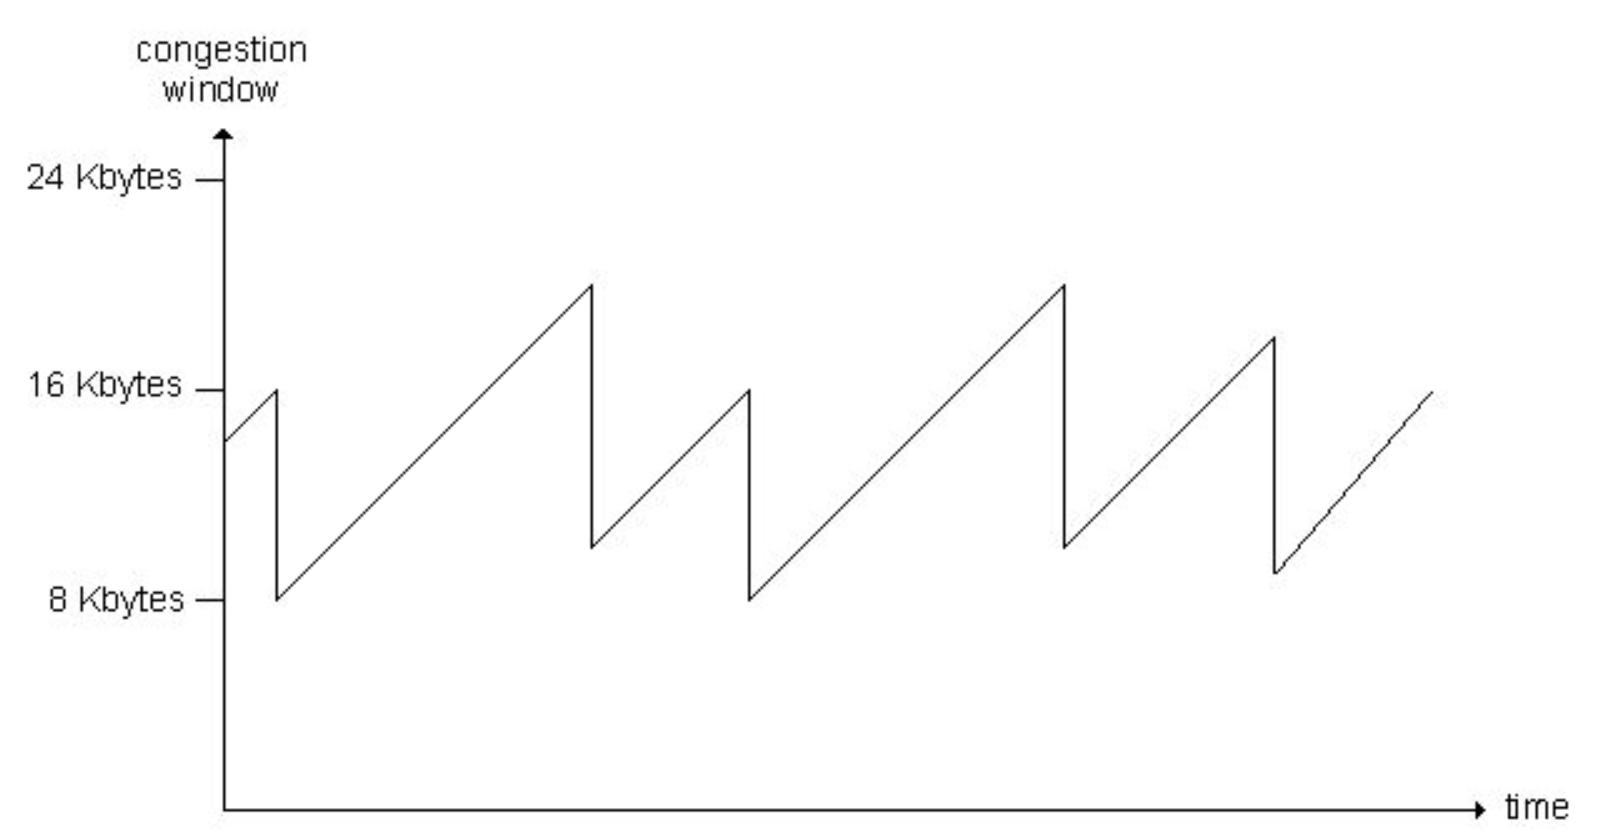
\includegraphics[page=1,scale=0.45]{AIMD.png}};
  \end{tikzpicture}
\caption{\textit{Presentación: Transport Layer: TCP Congestion Control $\&$ Buffer Management, Lilian Carroll, Slide 10}}
\end{figure}
\subsubsection*{Fast Retransmit and Recovery (FRR)}
Es un algoritmo de control de congestión que permite recuperar rápidamente los paquetes de datos perdidos. Sin FRR, el TCP requiere un temporizador que requiere un tiempo de espera si se pierde un paquete. Con FRR, si un receptor recibe un segmento que esta fuera de orden, inmediatamente envia un \texttt{ACK} duplicado al remitente. Si el remitente recibe 3 \texttt{ACK} supone que se perdió e inmediatamente retransmite el segmento perdido.

\subsection*{Versiones TCP}
\begin{itemize}
\item \texttt{TCP Tahoe}: Los primeros mecanismos fueron Slow Start y la estimación de \texttt{RTT}. Junto con la prevension de congestion y finalmente la Retransmisión Rápida. (\texttt{SS+AI+FR}). Tiene por lo tanto mecanismos basicos de congestión y recuperación de perdidas. El principal problema es el inicio lento concretamente en enlaces de retardo elevado.
\item \texttt{TCP Reno}: Se incorporan todas las características de Tahoe y se añade la \textbf{Recuperación Rapida}, que actua conjuntamente con el de Retransmision Rapida. De esta forma, tras la retransmision no se invoca Slow Start sino el de prevension de congestión. El inconveniente es cuando tenemos multiples perdidas por ventana, no se puede recuperar de forma rapida mas que la primera perdida. (\texttt{SS+AI+FRR})
\item \texttt{TCP New-Reno}: Es como el Reno pero con una modificación al algoritmo de Recuperacion Rapida (\texttt{Reno+Partical ACK}).
\item \texttt{TCP Vegas}: En esta modifican aspectos de los algoritmos de Retransmisión y Recuperación. Así como el inicio lento. Lo que hace es actuar contra la congestión antes que se detecte por la expiración del temporizador.
\item Otros: \texttt{TCP SACK} (Reno+Selective \texttt{ACK}) y \texttt{FACK} (Reno + Forward \texttt{ACK}).
\end{itemize} 
 

 
%\begin{figure}[H]
%\centering
%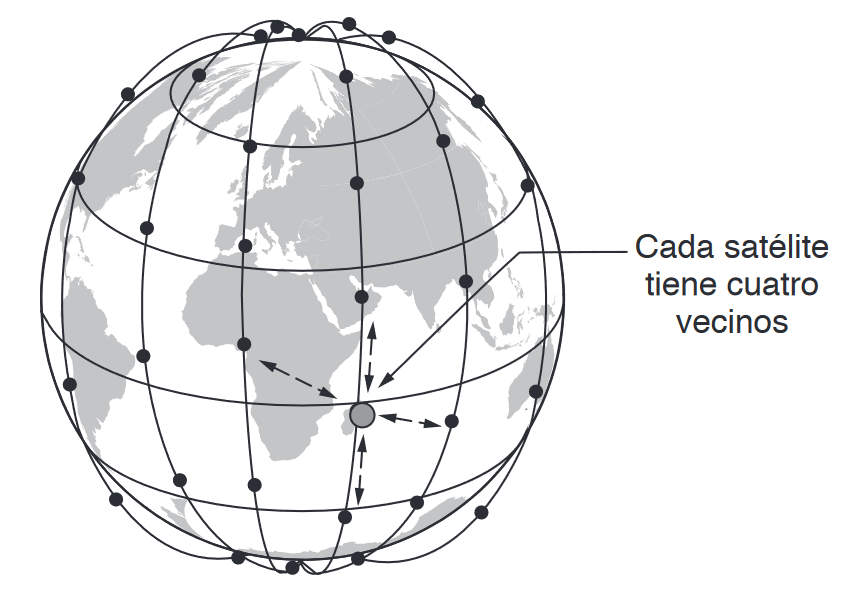
\includegraphics[page=1,scale=0.7]{SATELITES2.png}
%\caption{Satélites Iridium \textit{(Redes de Computadoras, Tanenbaum 4ta Edición, Pagina 105)}}
%\end{figure}

%\begin{figure}[H]
%\centering
%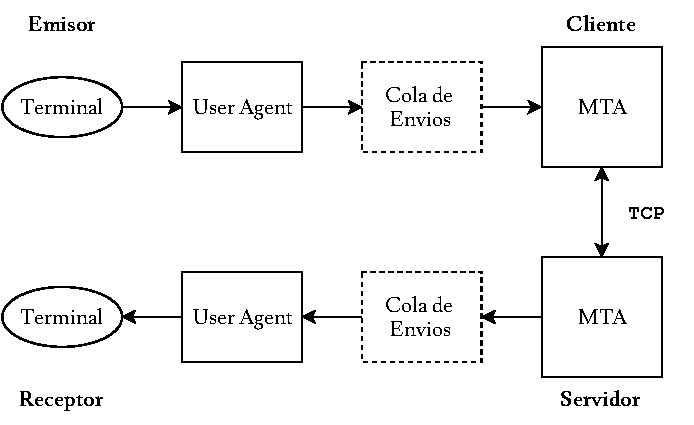
\includegraphics[page=1,scale=0.7]{SMTP.pdf}
%\caption{Esquema de funcionamiento de SMTP}
%\end{figure}
